\section{Analog Part: Fullwave rectifier}
\subsection{Fullwave rectifier}
A power supply uses a full-wave rectifier to convert a sinusoidal input signal into a dc voltage. The sinusoidal input voltage from the wall plugin is represented by $v_{ac}(t) = A\sin({\omega_1t})$ where  $\omega_1 = 120\pi$ and $A = 160V$. \newline\newline

The output of the full-wave rectifier used in this circuit is the absolute value of the sinusoidal input. The absolute value will be used to create a dc output voltage. Since the output of the rectifier is the absolute value of the input, all negative half cycles of the sinusoidal will be turned into positive half cycles. This causes the output to be a periodic signal with a fundamental frequency of $2\omega_1$. \newline

Periodic signals can be represented by Fourier series. The Fourier series of the periodic output signal of the full-wave rectifier will contain a dc component and some sinusoidal components. The Fourier series for the full-wave rectifier used in this circuit is represented by equations \ref{Fullwave_rectifier_1} to \ref{Fullwave_rectifer_6}.
\begin{equation}
    \label{Fullwave_rectifier_1}
    v_{ac}(t) = 160\sin(120\pi t)
\end{equation}

\begin{equation}
    \label{Fullwave_rectifier_T}
    T = \frac{2\pi}{240\pi} = \frac{1}{120}
\end{equation}

\begin{equation}
\label{Fullwave_rectifer_2}
   \begin{split}
a_0 &= \frac{1}{T} \int\limits_{}^{T} f(t)\: \mathrm{d}t \\
  &\quad120 \cdot 160 \int\limits_{n}^{\frac{1}{120}} \sin(120\pi t) \mathrm{d}t\\
  &\quad \frac{19200}{120\pi} [-\cos(120\pi t)]_{0}^{\frac{1}{120}} \\
  &\quad \frac{160}{\pi}[-(\cos(\pi)-\cos(0))]\\
  &\quad - \frac{160}{\pi} (-2) = \frac{320}{\pi}
\end{split} 
\end{equation}

\begin{equation}
\label{Fullwave_rectifer_3}
   \begin{split}
a_n &= \frac{2}{T} \int\limits_{}^{T} f(t)\: \cos(\omega_0 n t) \mathrm{d}t \\
  &\quad 240 \cdot 160 \int\limits_{0}^{\frac{1}{120}} \sin(120\pi t)\cos(240\pi n t) \mathrm{d}t\\
\end{split} 
\end{equation}

\begin{equation}
\label{Fullwave_rectifer_4}
      \sin(120\pi t)\cos(240\pi t) = \frac{1}{2}[\sin(120\pi t + 240\pi n t)+\sin (120 \pi t - 240 \pi n t)] =
   \frac{1}{2}[\sin(120 \pi t (1+2n))+ \sin(120 \pi t (1-2n))]  
\end{equation}
\begin{equation}
\label{Fullwave_rectifer_5}
    \begin{split}
        a_n &= \frac{38400}{2} \int\limits_{0}^{\frac{1}{120}} \sin(120 \pi t (1+2n))+ \sin(120 \pi t (1-2n)) \mathrm{d}t\\
        &\quad 19200 \int\limits_{0}^{\frac{1}{120}} \sin(120 \pi t (1+2n)) \mathrm{d}t + 19200 \int\limits_{0}^{\frac{1}{120}} \sin(120 \pi t (1-2n)) \mathrm{d}t\\
        &\quad \frac{-160}{\pi (1+2n)}[\cos(120\pi t(1+2n))]_{0}^{\frac{1}{120}} - \frac{160}{\pi (1-2n)}[\cos(120 \pi t (1-2n)))]_{0}^{\frac{1}{120}}\\
        &\quad \frac{-160}{\pi (1+2n)}(\cos(\pi(1+2n))-1)\frac{-160}{\pi(1-2n)}(\cos\pi(1-2n)-1)\\
        &\quad \frac{320}{\pi(1+2n)}+\frac{320}{\pi(1-2n)}-\frac{320\pi(1-2n)+320\pi (1+2n)}{\pi(1+n2)(1-2n)}\\
        &\quad \frac{32-\pi(1-2n+1+2n)}{\pi^2(1-4n^2)} = \frac{-640}{\pi(4n^2-1)}
    \end{split}
\end{equation}

\newline
The Fourier series results in the following expression for the periodic output signal. The dc component is represented by
\begin{equation}
     \frac{320}{\pi}  
\end{equation}
and the sinusoidal component is represented by 
\begin{equation}
  \displaystyle\sum_{n=1}^{N} \frac{640}{\pi(4n^2-1)}  
\end{equation}.
\newline
Therefor $v_s(t)$ can be written as shown in equation \ref{Fullwave_rectifer_6}.
\begin{equation}
\label{Fullwave_rectifer_6}
    v_s(t) = \frac{320}{\pi}- \displaystyle\sum_{n=1}^{N} \frac{640}{\pi(4n^2-1)}  
\end{equation}

\subsection{RL filter}
The RL filter must meet two specifications. The first one is that the output voltage has to be at least 90 Volts. The second one is that the output voltage has a maximum ripple of $5\%$. To meet the first specification the transfer function of the filter will be determined. 
The transfer function of the RL filter is given by equation \ref{RL_filter_1}. Where $V_{rectout}$ is the dc component of the Fourier series. \newline
\begin{equation}
\label{RL_filter_1}
\begin{split}
    V_{out} &= \frac{R}{R_S + R} \cdot V_{rectout} \\ 
    &\quad \frac{R}{R+10} \cdot \frac{320}{\pi}\\
\end{split}
\end{equation} 
\newline
Since the output voltage must be at least 90 Volts the following equations can be solved.

\begin{equation}
\label{RL_filter_2}
    \begin{split}
        \frac{R}{R+10} \cdot \frac{320}{\pi} \geq 90 \\
        320R \geq 90\pi R + 900\pi \\
        37,2566R \geq 900\pi\\
        R \geq 75,89 \Omega
    \end{split}
\end{equation}
To keep the output voltage at least at 90 Volts, there is chosen for $R = 100\Omgea$. 

\begin{equation}
  V_{out} = \frac{100}{110} \cdot \frac{320}{\pi} = 92,6V 
\end{equation}
The output voltage of $92,6V$ is achieved with the chosen resistor value witch is acceptable. \newline
To meet the second specification the steady-state response of $v_{sn}(t)$ needs to be determined. 

\begin{equation}
\label{RL_filter_3}
    V_{outn} = \frac{R}{R+R_2+njn\omega_1L} \cdot V_{sn}
\end{equation}

\begin{equation}
\label{RL_filter_4}
    V_{sn} = \frac{640}{\pi(4n^2-1)}
\end{equation}

By calculating the Fourier series the input sinusoidal is simply snapped at t = T and copied n-times. For that reason the most common harmonic is at n = 1. Next the inductance needs to be determined to meet the second specification at n = 1 by taking the absolute value of equation \ref{RL_filter_3}. The calculation of the inductance to meet the maximum of $5\%$ ripple is represented by equations \ref{RL_filter_3} to \ref{RL_filter_5}.  

\begin{equation}
\label{RL_filter_5}
    \begin{split}
        V_{out1} = \frac{100}{110 + j240\pi L}\cdot \frac{640}{3\pi} \\
        |V_{out1}| = \frac{100}{\sqrt{110^2 + (240\pi)^2 L^2}} \cdot \frac{640}{3\pi} \leq 0,05 v_{o1}\\
        v_{o1} = 92,6 V\\
        |V_{out1}| = \frac{6400}{3\pi} \leq 4,63\sqrt{110^2 + (240\pi)^2 L^2}\\
        (240\pi)^2 L^2 \geq 2138975,21\\
        L^2 \geq 3,625\\
        L \geq \sqrt{3,625} \\
        L \geq 1,9397 H
    \end{split}
\end{equation}\\

The value of the inductor (L) will be 2 Henry based on the calculations.

\subsection{Simulation}

\begin{figure}[!htb]
    \centering
    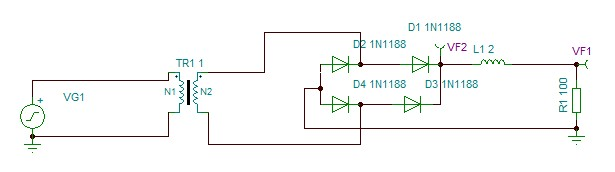
\includegraphics[width=0.8\textwidth]{figuren/Circuit_FWR.JPG}
    \caption{Circuit full-wave rectifier}
    \label{fig:circuit_FWR}
\end{figure}

The circuit shown in figure \ref{fig:circuit_FWR} is used for the simulation of the full-wave rectifier. The diodes used in the simulation are selected on the amount of voltage they can handle. The diodes that are used in the simulation can handle up to 400 volt. 

\begin{figure}[!htb]
    \centering
    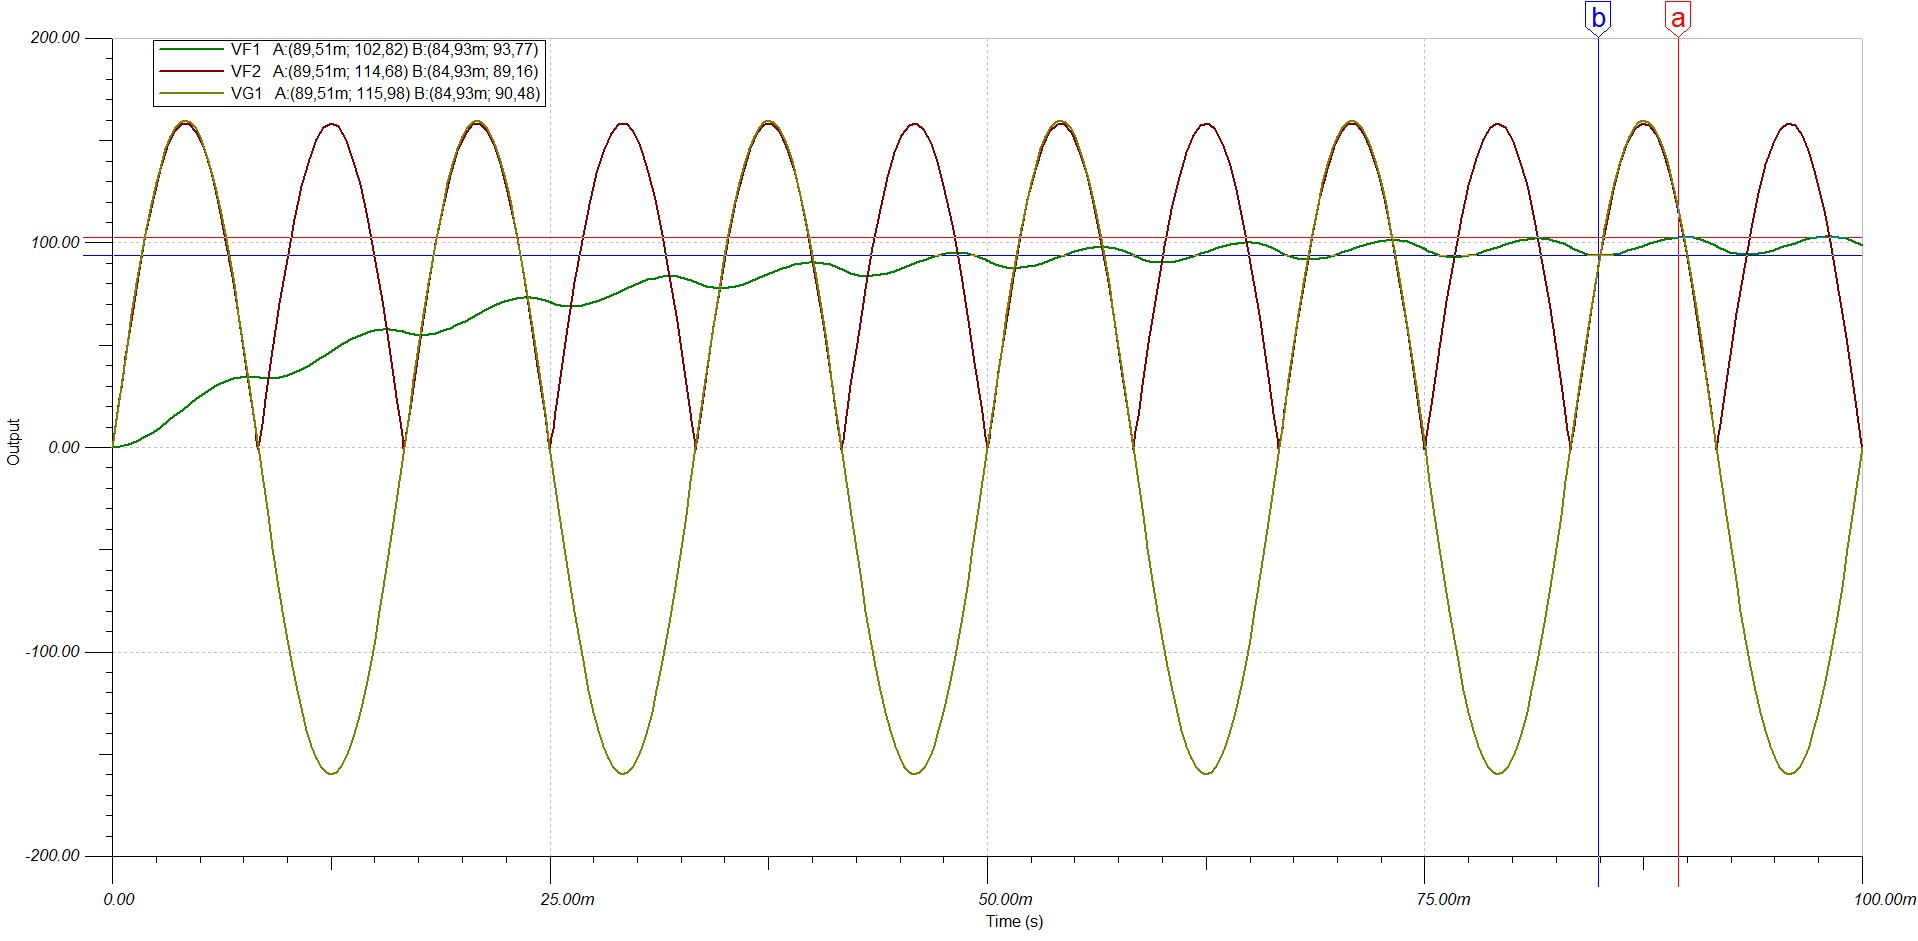
\includegraphics[width=0.8\textwidth]{figuren/Simulation_FWR.jpg}
    \caption{Simulation full-wave rectifier}
    \label{fig:Simulation_FWR}
\end{figure}

In figure \ref{fig:Simulation_FWR} is the simulation of the full-wave rectifier shown. Here is VF1 the output voltage, VG1 is the input voltage and VF2 is the rectified signal. The simulation shows that the two specifications are met. So is the minimum voltage 93,77 and the maximum voltage 102,82. This concludes that the voltage has a ripple of $4,4\%$.